\chapter{Giới thiệu hàm Lambert}
	\section{Giới thiệu}       
		Hàm Lambert $W$ được định nghĩa là một hàm phức ngược đa trị của hàm $w \mapsto we^{w}$ với $w \in \mathbb{C}$. Hàm này có rất nhiều ứng dụng trong cả toán thuần túy và toán ứng dụng và một trong số chúng sẽ được trình bày trong mục 2.2 dưới đây. \\    
		Năm 1758, Lambert nghiên cứu phương trình $x = q + x^{m}$ với ẩn số x. Trong [1], Euler biến đổi phương trình Lambert về dạng đối xứng hơn \begin{align}x^{\alpha} - x^{\beta} = (\alpha - \beta)vx^{\alpha + \beta} \end{align}
 bởi thay thế $x = x^{-\beta}$ và đặt $m = \frac{\alpha}{\beta}$ và $q = (\alpha - \beta)v$.
		Phiên bản Euler của chuỗi Lambert có dạng sau 
		\begin{align}
			\begin{split}
				x^{\gamma} = 1 + \gamma v + \frac{1}{2}\gamma(\gamma + \alpha + \beta)v^{2} + \frac{1}{6}\gamma(\gamma + \alpha + 2\beta)(\gamma + 2\alpha + \beta)v^{3} \\ + \frac{1}{24}\gamma(\gamma + \alpha + 3\beta)(\gamma + 2\alpha + 2\beta)(\gamma + 3\alpha + \beta)v^{4} + ...
			\end{split}
		\end{align}
	Sau khi chuyển đổi chuỗi, Euler nhìn vào trường hợp đặc biệt, bắt đầu từ $\alpha = \beta$. Để nhìn thấy ý tưởng từ phương trình ban đầu, ta chia (1.1) cho $(\alpha - \beta)$ và cho $\beta \rightarrow \alpha$, ta được
		\begin{align*}
			\displaystyle \lim_{\beta \to \alpha}\frac{x^{\alpha}-x^{\beta}}{\alpha - \beta} = vx^{2\alpha}\\
			\mbox{Do đó } x^{\alpha}\log \alpha = vx^{2\alpha}
		\end{align*}
		\begin{align}
			\mbox{Vì vậy } \log x = vx^{\alpha}
		\end{align}
	Euler chú ý rằng nếu chúng ta giải được phương trình (1.3) với $\alpha = 1$ thì chúng ta có thể giải được nó với mọi $\alpha \neq 0$. Để thấy điều này,ta nhân phương trình (1.3) với $\alpha$,dẫn đến $\alpha \log x = \log x^{\alpha}$. Đặt $z = x^{\alpha}$ và $u = \alpha v$, ta có $\log z = u z$ là kết quả phương trình (1.3) với $\alpha = 1$. \\
	Để giải phương trình (1.2), đầu tiên Euler cho $\alpha = \beta = 1$ và viết lại (1.2) dưới dạng chuỗi của $\frac{x^{\gamma}-1}{\gamma}$. Từ phương trình (1.2) thì 
		\begin{align*}
			\frac{x^{\gamma}-1}{\gamma} = v + \frac{1}{2}(\gamma+2)v^{2} + \frac{1}{6}(\gamma+3)(\gamma+3)v^{3} + ... 
		\end{align*}
		Tiếp đến, ông cho $\gamma \rightarrow$ 0, vì \begin{align*} \displaystyle \lim_{\gamma \to 0}\frac{x^{\gamma}-1}{\gamma} = \log x 
		\end{align*}
		\begin{align} \mbox{nên ta thu được }\log x = v + \frac{2^{1}}{2!}v^{2} + \frac{3^{2}}{3!}v^{3} + \frac{4^3}{4!}v^{4} + ... 
		\end{align}
		Chuỗi này hội tụ với $|v| < \frac{1}{e}$,nó được định nghĩa là hàm $T(v)$ gọi là hàm cây [2]. Nó có giá trị bằng với $-W(-v)$ với $W(z)$ được định nghĩa là hàm thỏa mãn 
		\begin{align}
			W(z)e^{W(z)} = z.
		\end{align} 
		Chúng ta sẽ gọi tắt 2 hàm này là $T$ và $W$. Hai hàm này được sử dụng trong rất nhiều ứng dụng như : liệt kê số cây $[3,4]$, tính toán độ cao cột nước $[5]$ và trong bài toán được xem xét bởi Pólya và Szego $[6]$.Wright sử dụng nhánh phức của hàm $W$ và tính tổng quát của hàm mũ để tính toán phương trình vi phân có trễ hệ số hằng.\\
		Hàm Lambert $W$ là hàm có giá trị phức tạp, cùng với đối số phức tạp $z$ và nó có vô hạn nhánh $W_{k}$, ở đó $k = -\infty, ..., -1, 0 , 1, \infty$. Đường thẳng thực của nhánh chính của hàm Lambert $W$ ,$W_{0}$ có giá trị nhỏ nhất là -1. Nhánh chính và tất cả các nhánh khác của hàm Lambert có thể được tính toán giải tích thông qua việc tính toán chuỗi. Các ngôn ngữ tính toán khoa học phổ biến hiện nay như Python, Matlab, Maple, Mathematica, ... đều có hàm Lambert (vô hướng) dựng sẵn với độ chính xác tùy ý.
\begin{verbatim}
syms x
fplot(lambertw(x))
hold on
fplot(lambertw(-1,x))
hold off
axis([-0.5 4 -4 2])
title('Hàm Lambert W , 2 nhánh chính')
legend('k=0','k=-1','Location','best')
\end{verbatim}
\begin{figure}
	\centering
    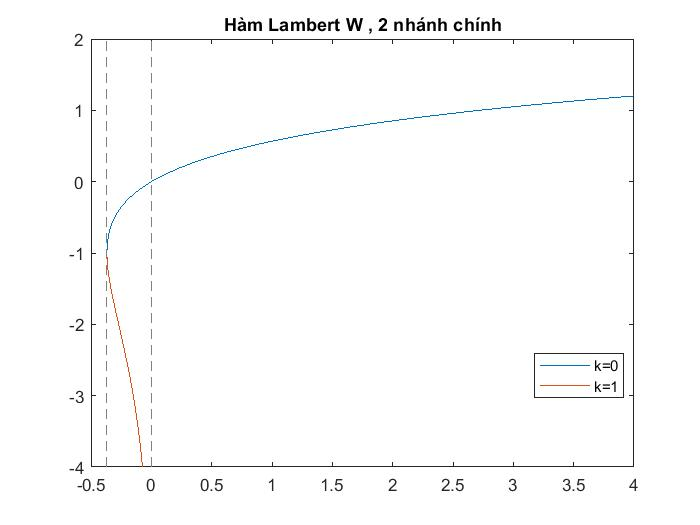
\includegraphics[scale=0.5]{MATLAB_files/wfig.jpg}
    \caption{Hàm Lambert với 2 nhánh chính k=0, k=-1}
\end{figure}

